\documentclass[12pt]{article}


\usepackage{amssymb}
\usepackage{amsmath}
\usepackage[utf8]{inputenc}
\usepackage[ngerman]{babel}
\usepackage{lineno}
\usepackage{listings}
\usepackage[T1]{fontenc}
\usepackage[utf8]{inputenc}
\usepackage{lmodern}
\usepackage{eurosym}
\usepackage{listings}
\usepackage{microtype}
\usepackage{units}
\usepackage{color}
\usepackage{xcolor}
\usepackage{graphicx}
\usepackage{subfigure}
\usepackage{import}
\usepackage{url}
\usepackage{amsthm}
\theoremstyle{plain}

\lstset
{ %
  language=R,                     % the language of the code
  basicstyle=\footnotesize\ttfamily,       % the size of the fonts that are used for the code
  numbers=left,                   % where to put the line-numbers
  numberstyle=\tiny\color{gray},  % the style that is used for the line-numbers
  stepnumber=1,                   % the step between two line-numbers. If it's 1, each line
                                  % will be numbered
  numbersep=5pt,                  % how far the line-numbers are from the code
  backgroundcolor=\color{white},  % choose the background color. You must add \usepackage{color}
  showspaces=false,               % show spaces adding particular underscores
  showstringspaces=false,         % underline spaces within strings
  showtabs=false,                 % show tabs within strings adding particular underscores
  frame=single,                   % adds a frame around the code
  rulecolor=\color{black},        % if not set, the frame-color may be changed on line-breaks within not-black text (e.g. commens (green here))
  tabsize=2,                      % sets default tabsize to 2 spaces
  captionpos=b,                   % sets the caption-position to bottom
  breaklines=true,                % sets automatic line breaking
  breakatwhitespace=false,        % sets if automatic breaks should only happen at whitespace
  title=\lstname,                 % show the filename of files included with \lstinputlisting;
                                  % also try caption instead of title
%  keywordstyle=\color{blue},      % keyword style
%  commentstyle=\color{green},   % comment style
%  stringstyle=\color{blue},       % string literal style
  %escapeinside={\%*}{*)},         % if you want to add a comment within your code
  escapeinside={(*@}{@*)},         
  morekeywords={*,...}            % if you want to add more keywords to the set
} 

\title{default title}
\author{default author \\facculty}
\date{00/00/0000}

\begin{document}
\pagenumbering{arabic}
\maketitle
\centerline{\rule{1.2\linewidth}{.2pt}}
\begin{linenumbers}
\section{Konzept}
-GOGOL (kurz für Game of Game of Life) ist eine Desktop Applikation für das berühmte nullspieler-spiel
Game of Life, welches vom britischen mathematiker John Horton Conway im jahr 1970 entwickelt wurde.
- das grundkonzept des spiels besteht aus einem zweidimensionalen, rechteckigen gitter, wobei jedes feld in diesem gitter einer zelle entspricht
- eine zelle kann pro generationsschritt einen von zwei zuständen haben: lebend, tot
- der zustand einer zelle ist abhängig von den 8 nachbarn die, die zelle umgeben
- bei einem generationsübergang wird nun der zustand einer zelle bestimmt:
- Eine tote Zelle mit genau drei lebenden Nachbarn wird in der Folgegeneration neu geboren.
-Lebende Zellen mit weniger als zwei lebenden Nachbarn sterben in der Folgegeneration an isolation.
- Eine lebende Zelle mit zwei oder drei lebenden Nachbarn bleibt in der Folgegeneration am Leben.
- Lebende Zellen mit mehr als drei lebenden Nachbarn sterben in der Folgegeneration an Überbevölkerung.

Aus diesen einfach regeln enstehen verblüffende strukturen, welche einzigartige verhaltensmuster, bishin zur turing-completeness aufweisen.

Die Grundidee war das entwickeln einer soliden desktop anwendung die weitere nützliche bedienfunktionen hat.
Darüber hinaus soll das programm, neben dem standart spiel noch weitere modi zu implementieren, welche eine abwandlung des "vanilla" GoL bieten.
Zu anfangs geplant waren:
standard conway
colormerge - das verschmelzen von zellen mit farbeigenschaften
colorwar - kampf von zellen mit "teamfarben"
probability of life - random warscheinlichkeit bei der geburt von zellen

zuletzt sollte noch ein lokaler player versus player modus implementiert werden, welcher der anwendung seinen eigentlichen namen verleiht, da so auf dem game of life ein tatsächliches spiel ensteht

Sinn der applikation besteht darin, aus dem game of life einen unterhaltungswert zu gewinnen und somit eine beschäftigung für zwischendurch zu schaffen

\section{Planung}

\subsection{meilensteine}
idee war es die jeweiligen features in meilensteine zu unterteilen sobald eine primitive version des spiel besteht, die meilensteine wurden dann 1:1 auf sprints aufgeteilt die alle 1 oder 2 wochen länge hatten,
je nach vermutung der workload, so enstanden zu nächst folgende meilensteine und sprints:
-grundimplementation: 1. primitive laufende version
-automatisierung: qol- features wie: play/stop, speedregler, load/save, preloaden von strukturen sog. species
-rainbow: custom rules, colormerge, colorwar
-bio: probability of life
-pvp: exterminate, populate
-dokumentation
-website: deployment einer einfachen webseite zum hosten der anwendung als web-applet oder bereitstellen zum download

wir haben gfrundfunktionalitäten priorisiert da höhere funktionalitäten suksessiv auf niedrigere features aufbauen,
höhere funktionen wäre ohne vorherige implementation der vorherigen grundfunktionen nicht lauffähig

\subsection{zeitplan}
die sprints haben zueinander einen critical path, jedoch war theoretisch die abgabe schon nach dem abschließen der automatisierung möglich
für die abgabe war der plan, eine woche vor deadline fertig zu sein um bei auftretenden problemen einen puffer zu haben
\newline
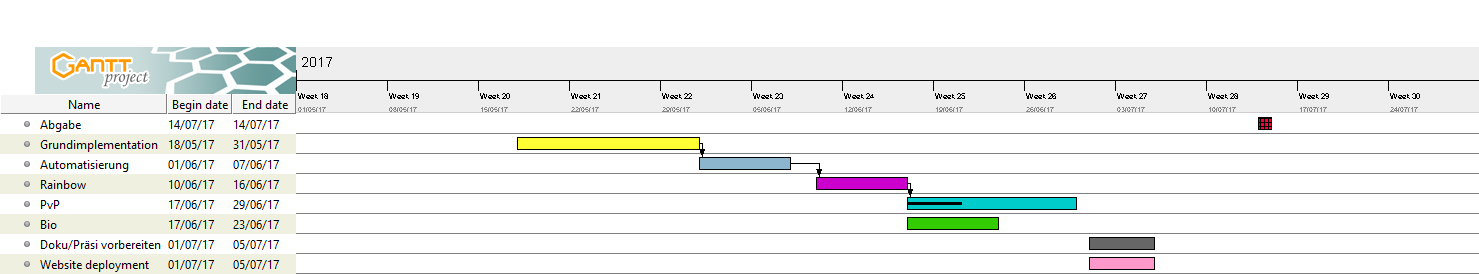
\includegraphics{images/ganttdep.png}
\newline
der erste entwurf des gant diagrams

wie hat sich die planung im laufe des projekt verändert?
aufgrund von fehlerhaften schätzungen wurden subfeatures und einige meilensteine komplett entfernt oder verschoben

demnach veränderte sich der projektverlauf
siehe auch: was wurde verworfen
\newline
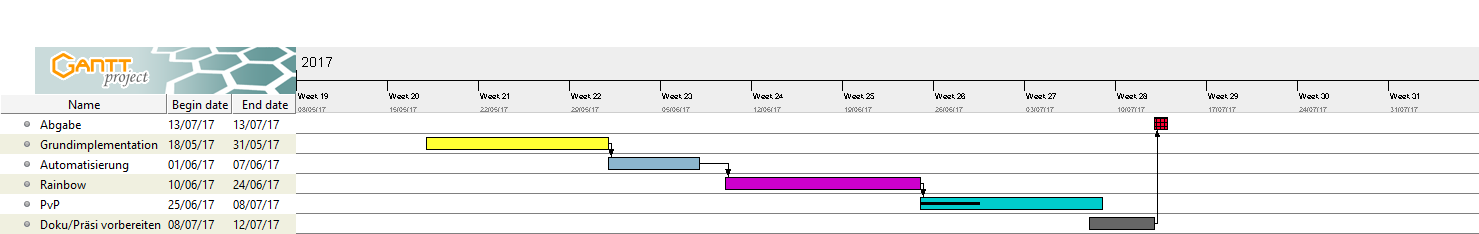
\includegraphics{images/gant.png}
\newline
letzte aktuelle version der planung

\subsection{testplan}

tests wurden dem jeweiligen sprint zugeteilt und nach fertigstellung der features implementiert
mit ausnahme von rainbow, dort wurde ein test first ansatz verwendet

\subsection{technische beschreibung des systems}

die systemarchitektur liegt dem MVC (Model, View, Controller)-Ansatz zugrunde:
Der View-teil besteht aus einem GUI, sowie einem Gamegrid, welches an das GUI übergeben wird und dieses darstellt.
Das GUI hält das gamegrid lediglich als container und führt keine sondierenden methoden auf dem gamegrid aus.
Als Model-Teil wurden zunächst die Zellen implementiert, diese halten keine logik sondern geben nur ihren status nach außen oder kriegen ihre eigenschaften
von außen gesetzt. Die Zellen werden dann in einem 2 dimensionalen array: der survivalmatrix, gesetzt. Desweiteren gibt es ein Regelwerk hier: Ruler,
dieser hält alle methoden der spielregeln und gibt das cellverhalten vor, welche vom controller dann verwendet werden. Für den PvP modus ist ein Referee zuständig der die 2spielerreglen
verwaltet. Für das preloaden der species wurde ein species model entwickelt, welches die eigenschaften für die SVM hält und in einer specieslibrary verwaltet wird. der Preloader wendet diese auf die SVM an.
Hauptkomponente des Controller-teils stellt der Controller dar, dieser hält alle logikteile, die wiederum doe modelle halten. er hält außerdem als einziger die SVM.
des weiteren kriegt er bei seiner erstelluing das gamegrid und das gui überreicht. daher ist er für die verwaltung zuständig, er stellt verbindung zwischen logik und gui her in dem
er alle listener erstellt und an die buttons bindet.
\newline
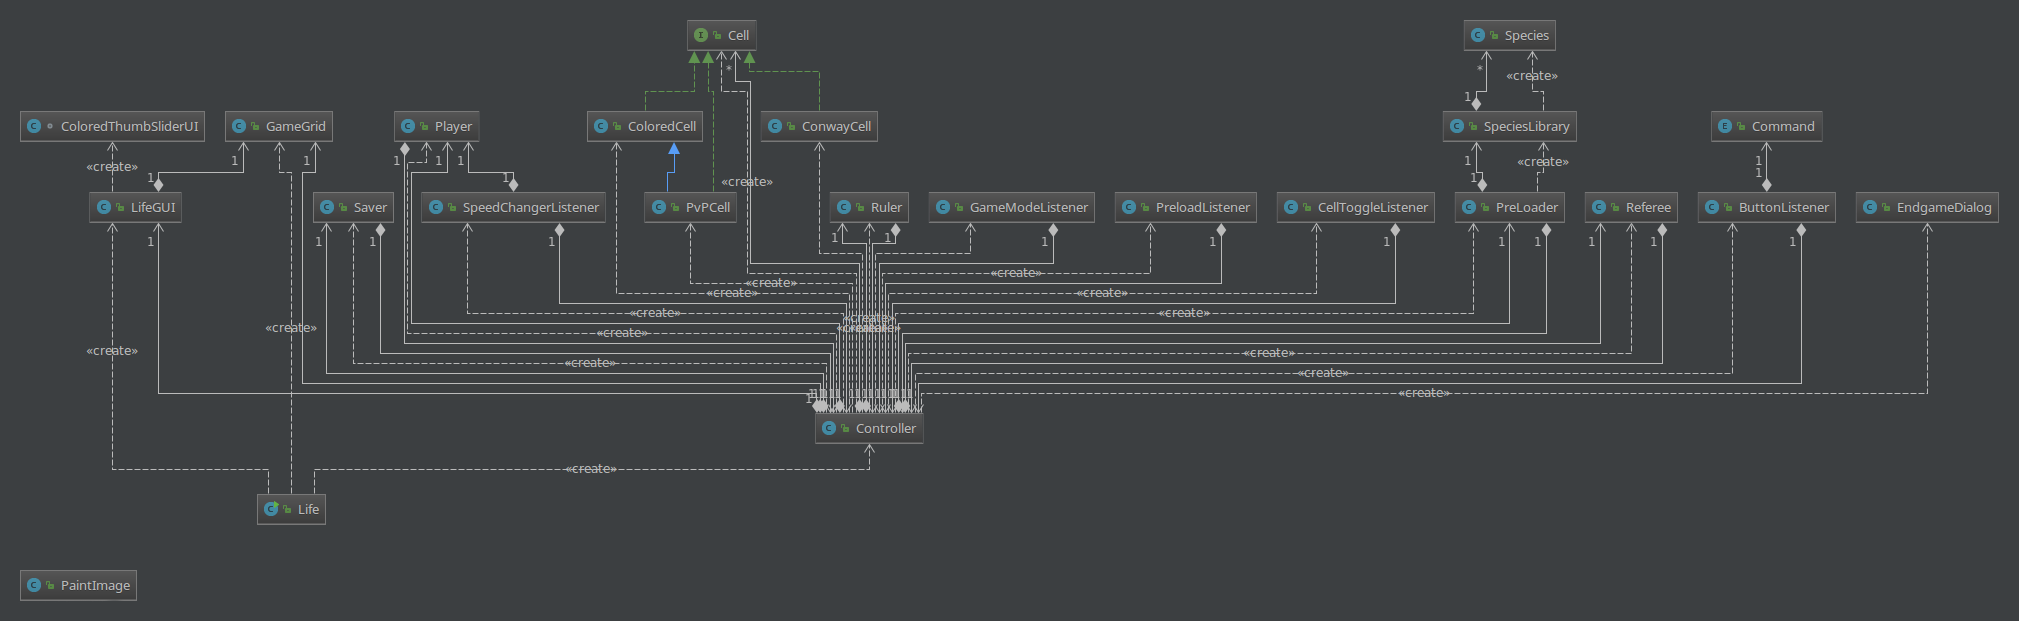
\includegraphics{images/gogolClasses.png}
\newline
als kapselung wurden die klassen in mehrere packages unterteilt und somit ihrer funktionalität unterteile:
frontend:
SLiderUI
EndgameDialog
Gamegrid
LifeGui
PaintImage

backend:
command
controller
player
referee
ruler
saver

cells:
cell
coloredcell
conwaycell
pvpcell

library:
preloader
species
specieslibrary

listener:
buttonlistener
celltogglelistener
gamemodelistener
preloadlistener
speedchangerlistener
\newline
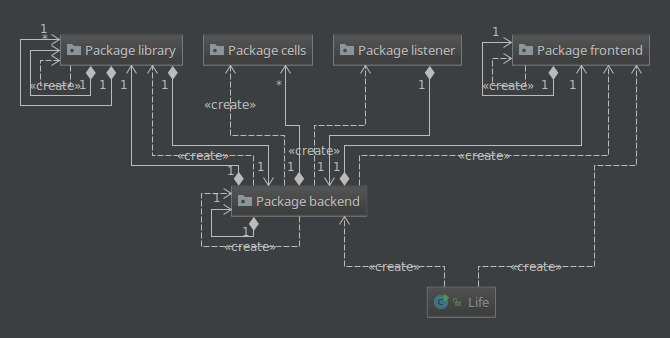
\includegraphics{images/gogolPackages.png}
\newline

\section{stand des projekts}
% STAND DES PROJEKTS
\subsection{Was ist fertig?}
% was ist fertig?
Das klassische Game of Life nach Conway ist vollständig, sowie die alternativen Spielmodi ColorMerge, ColorWar und PvP.
Für jeden dieser Modi sind die Funktionalitäten Speichern/Laden des aktuellen Spielstandes, laden bestimmter Presets, sowie (ausgenommen für den Modus PvP) eine zufällige Initialisierung des Spielfeldes.
\subsection{Verworfen}
% was wurde verworfen(warum)?
\begin{itemize}
\item
Der geplante Modus Propability of Life wurde verworfen. Dieser hätte beinhaltet, dass Zellen abhängig von ihrer Anzahl Nachbarn eine bestimmte Wahrscheinlichkeit haben in der nächsten Generation lebend oder tot zu sein. Das Zellverhalten wäre somit jedoch nicht mehr deterministisch. Eine Nutzung der Presets oder das eigene finden bzw. erstellen solcher wäre in diesem Modus somit unmöglich, womit der entscheidende Aspekt des Game of Life verloren gegangen wäre. Auch wenn die Idee interessant ist, hat sie keinen Bezug zu dem Game of Life und den restlichen Spielmodi.
\item
Der geplante Modus PvP - Exterminate wurde verworfen. In diesem PvP Modus wäre is das Ziel gewesen möglichst viele Zellen des Gegners zu vernichten. Schon die Definition wann eine Zelle vernichtet oder einfach nur abgestorben ist gestaltet sich als schwierig und wäre für die Spieler schwer verständlich und während des Spiels nicht in realistischer Zeit nachvollziehbar.
\item
Das geplante Feature Custom Ruleset wurde verworfen. Dieses hätte dem Spieler ermöglicht die Bedingungen, bei wievielen Nachbarn eine Zelle lebend oder tot sein wird anzupassen. Dadurch werden jedoch Presets nicht mehr nutzbar, da diese auf dem Verhalten nach den Conway regeln beruhen, womit ein wichtiges Feature in diesem Modus vom User nicht erwartete Ergebnisse erzeugt hätte.
\item
Das Feature Change Gridsize ist momentan nicht nutzbar. Die Funktionalität ist bereits implementiert, jedoch ist kein Button auf der Öberfläche implementiert. Grund hierfür ist mangelnder Platz und nicht ausreichend Zeit um die GUI zu refactorn und welchen zu schaffen. In zukünftigen Patches wird dieses Feature vermutlich aufgenommen.
\item
Das geplante großflächige Bereitstellen von Presets ist momentan noch nicht nutzbar. Geplant war aus http://conwaylife.appspot.com/library die bekannten Presets per Webscraping auszulesen. Dies ist erfolgreich implementiert, redoch wird der code wir einzelne Presets nicht korrekt interpretiert, wodurch diese falsch dargestellt werden.  Des Weiteren gestaltet es sich schwer die große Menge an Presets für den User übersichtlich darzustellen. In zukünftigen Patches wird dieses Feature vermutlich aufgenommen.
\item
Überlegungen zur Verbesserung der Effizienz bei der Zustandsberechnung der Zellen wurden noch nicht implementiert. Grund hierfür sind mangelnde Zeit und bereits ausreichend gute Performance der Anwendung. In zukünftigen Patches wird die Effizienz vermutlich verbessert.
\end{itemize}

\subsection{Bekannte Bugs und Probleme}
% wo gibt es macken?
Bisher sind keine Bugs bekannt. Ein bekanntes Problem ist, dass der SpeedSlider eine Exponentielle Funktion für die Geschwindigkeit verwendet. Diese liefert zwar die gewünschte Funktionalität, ist jedoch weniger intuitiv als eine Lineare Funktion. Aufgrund geringer Priorität wird diese Anpassung in zukünftigen Patches durchgeführt.
\subsection{Workload}
% wie war die workload?
Die Workload des Meilensteins "Rainbow" wurde deutlich unterschätzt. Grund hierfür waren unterschiedliche Interpretationen der Methodendefinition. Hier raus resultierten Fehler im Verständnis der vom jeweils anderen geschriebenen Methoden und falsche Anwendung dieser. Anstatt einer Woche waren hier zwei Wochen nötig. Die Workload des Meilensteins "PvP" wurde überschätzt. In diesem Meilenstein konnte sein sehr großer Teil der Funktionalität auf dem Modus ColorWar aus dem vorherigem Meilenstein "Rainbow" aufgebaut werden. Anstelle der geplanten zwei Wochen wurde weniger als eine Woche benötigt.
\subsection{Arbeitsaufteilung}
% aufteilung in der gruppe
Die folgenden Aufgaben wurden von Kolja Hopfmann und Jonas Sander gemeinsam durchgeführt: Projektplanung, Implementierung der Klassen Controller und Referee.
Die folgenden Aufgaben wurden von Kolja Hopfmann übernommen: Projektmanagement, Implementierung der Packages Frontend und Listener, Implementierung der Klasse Player und des Commandhandling im Backend.
Die folgenden Aufgaben wurden von Jonas Sander übernommen: Implementierung der Packages Testing, Cells und Library, sowie die Implementierung der Klassen Saver und Ruler im Backend.
\section{Funktionsbeschreibung}
% FUNKTIONSBESCHREIBUNG
% kurze Bedienungsanleitung (Start, Ende, wichtige Menüs, Parameter, Vorgehensweise, ...)
% systemvorraussetzungen, installation
\subsection{Installation und Systemvorraussetzungen}
be stuff here
\newpage
\subsection{Bedienungsanleitung}
% ggfs. Screenshots der Programmfenster

Die Anwendung wird durch Ausführen der EXE (Windows) bzw. JAR (Linux) gestartet. Zu sehen ist das Anwendungsfenster.
\newline
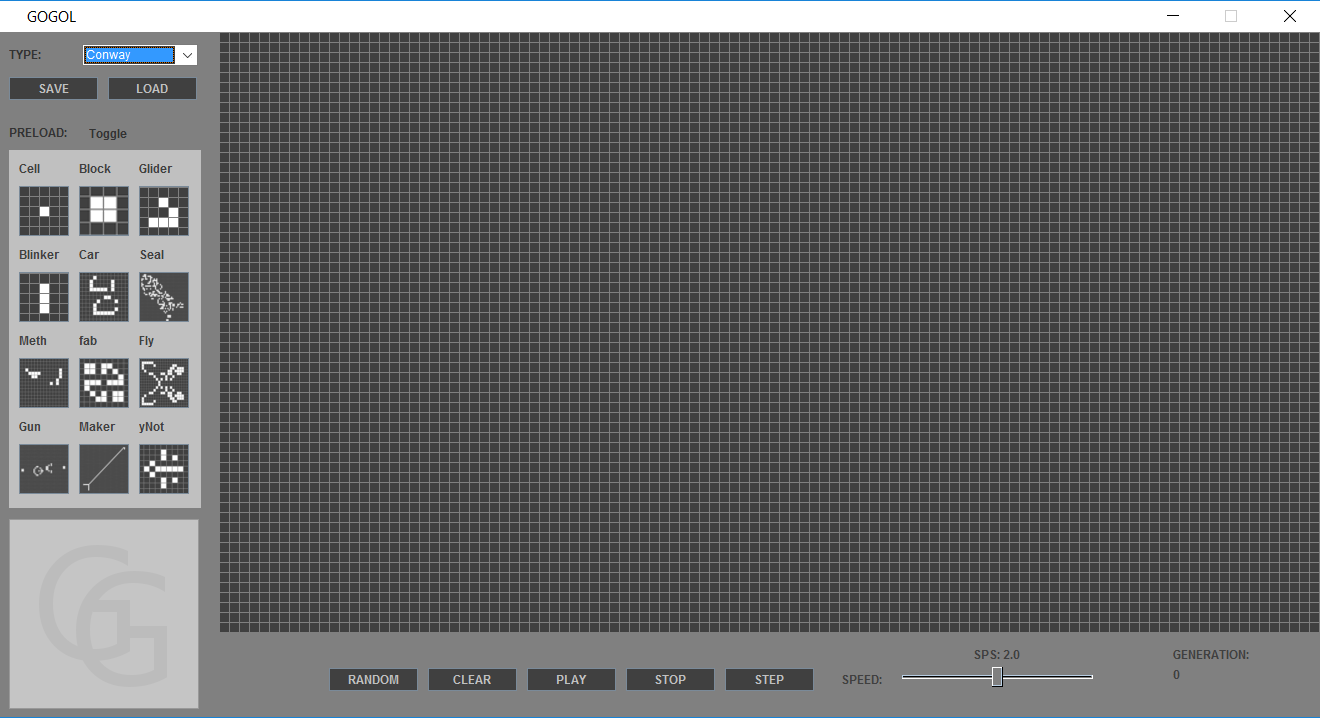
\includegraphics[scale=0.5]{images/manual_fullWindow.PNG}
\newline
Der größte teil ist das Spielfeld. Jedes Quadrat auf dem Spielfeld ist eine Zelle. Zellen können durch anklicken mit dem linken Mausknopf verändert werden (siehe Spielmodi).
\newline
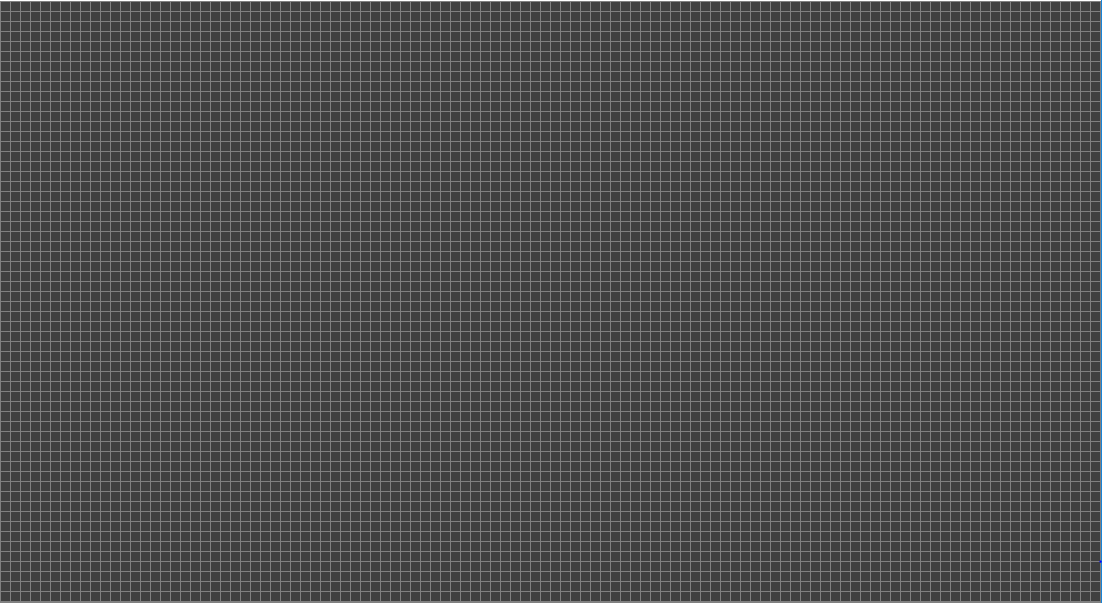
\includegraphics[scale=0.6]{images/manual_gamegrid.PNG}
\newline
Über das Dropdown Menü "TYPE" links oben kann der Spielmodus gewechselt werden (siehe Spielmodi). Beim Wechsel des Spielmodus wird das Spielfeld gleichzeitig auch immer geleert.
\newline

\includegraphics{images/manual_gamemode.PNG}
\newline
Mit dem Knopf "SAVE" kann der aktuelle Spielstand gespeichert werden. Über den Knopf "LOAD" kann ein früherer Spielstand geladen werden. Hierbei wird automatisch auf den entsprechenden Spielmodus gewechselt und ggf. die Spielfeldgröße angepasst.
\newline

\includegraphics{images/manual_saveload.PNG}
\newline
Das feld "PRELOAD: " gibt an auf welche Art Zellen momentan gesetzt werden. Toggle steht hierbei das Setzen einer einzelnen Zelle. Ist ein Preset ausgewählt, wird dessen Name angezeigt.
\newline

\includegraphics{images/manual_preloadMode.PNG}
\newline
Auf den verschiedenen Preset-Knöpfen ist die Zellbelegung des Jeweiligen Presets angezeigt, sowie dessen Name. Durch klicken eines Preset-Knopfes wird dieses Preset ausgewählt. Wird nun eine Zelle auf dem Spielfeld geklickt, wird dort das entsprechende Preset automatisch geladen. Presets sind besondere Strukturen, die jeweils ein bestimmtes Verhalten haben.
\newline
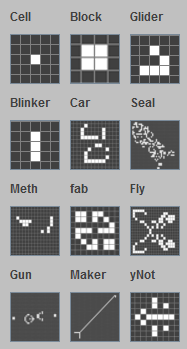
\includegraphics{images/manual_presets.PNG}
\newline
Über die Kontrollknöpfe kann das Spiel gesteuert werden. "RANDOM" belegt alle Zellen des Spielfeldes mit zufälligen Werten (siehe Spielmodi).
"CLEAR" leert das Spielfeld. "STEP" bringt das Spiel um eine Generation voran. "PLAY" lässt das Spiel automatisch eine bestimmte Anzahl Schritte pro Sekunde voranschreiten. "STOP" hält ein automatisch laufendes Spiel an. Im Spielmodus "PvP" ist das Verhalten der Knöpfe leicht verändert (siehe Spielmodi).
\newline

\includegraphics{images/manual_controlButtons.PNG}
\newline
SPS gibt die Anzahl Schritte an, die pro Sekunde bei einem Automatisch laufendem Spiel durchgeführt werden. Über den Slider kann die SPS angepasst 
werden.
\newline

\includegraphics{images/manual_speed.PNG}
\newline
Generation gibt die Aktuelle Zellgeneration des Spiels an. Bei jedem leeren des Spielfeldes, einer Zufallsbelegung und beim Wechseln des Spielmodus wird die Generation auf 0 zurückgesetzt.
\newline

\includegraphics{images/manual_generation.PNG}

\subsection{Spielmodi}
\subsubsection{Conway}
Dieser Spielmodus bietet das originale Game of Life nach Conway mit einigen Features zur vereinfachten Benutzung. Conways Game of Life ist ein Null-Spieler-Spiel. Der Spieler kann hier das Spielfeld nur bei Beginn einmalig modifizieren und danach das Zellverhalten beobachten. In unserer Version von Game of Life ermöglichen wir auch den späteren eingriff in das Spiel nach jeder Generation. Jede Zelle ist entweder tot oder lebendig. In jeder Generation wird für jede Zelle neu berechnet ob sie tot oder lebendig ist.
\begin{itemize}
\item Eine tote Zelle mit genau drei lebenden Nachbarn wird in der Folgegeneration neu geboren.
\item Lebende Zellen mit weniger als zwei lebenden Nachbarn sterben in der Folgegeneration an Isolation.
\item Eine lebende Zelle mit zwei oder drei lebenden Nachbarn bleibt in der Folgegeneration am Leben.
\item Lebende Zellen mit mehr als drei lebenden Nachbarn sterben in der Folgegeneration an Überbevölkerung.
\end{itemize}
Ein klick auf eine Zelle änderte den Status der Zelle zwischen lebendig und tot. Tote Zellen sind dunkel grau, lebendige Zellen sind weiß.

\subsubsection{ColorMerge}
In diesem Spielmodus erhält jede Zelle zusätzlich eine Farbe. Ob eine Zelle lebendig oder tot ist wird nach den selben Regeln wie im Spielmodus "Conway" bestimmt. Die Farbe einer neu geborenen Zelle berechnet sich durch den Mittelwert der Farben ihrer Nachbarzellen. Durch klick auf eine Zelle wird ihr Status wie Folgt geändert:
\newline
tot => lebendig, rot => lebendig, grün => lebendig, blau => tot => ...
\newline
Ein klick auf eine Zelle mit einer gemischten Farbe ändert diese zu lebendig, rot. Der Knopf "RANDOM" weist jeder Zelle zufällig einen Status lebendig oder tot zu, sowie jeder lebendigen Zelle eine Zufällige Farbe Rot, Grün oder Blau.

\subsubsection{ColorWar}
In diesem Spielmodus erhält wie in "ColorMerge" jede Zelle eine Farbe. Ob eine Zelle tot oder lebendig ist, wird weiterhin nach den selben Regeln wie im Spielmodus "Conway" bestimmt, jedoch mit einem Zusatz für die Geburt neuer Zellen. Wird eine Zelle neu geboren, muss es unter den Nachbarn eine Farbe mit eindeutiger Zellmehrheit geben, damit eine Zelle geboren werden kann. Die Farbe der neu geborenen Zelle ist immer identisch mit der mehrheitlichen Farbe der Nachbarzellen.
\newline
Durch klick auf eine Zelle wird ihr Status wie Folgt geändert:
\newline
tot => lebendig, rot => lebendig, grün => lebendig, blau => tot => ...
\newline
Der Knopf "RANDOM" weist jeder Zelle zufällig einen Status lebendig oder tot zu, sowie jeder lebendigen Zelle eine Zufällige Farbe Rot, Grün oder Blau. Werden in geladene Presets Zellen mit anderer Farbe gesetzt, verliert die Struktur möglicherweise ihre Funktionalität.

\subsubsection{PvP}
Dieser Spielmodus konvertiert Conways Game of Life in ein tatsächliches 2-Spieler-Spiel und ist Namensgeber für die Applikation GOGOL (Game of Game of Life). "PvP" beruht auf dem Spielmodus "ColorWar". Hier gibt es nun jedoch einen roten Spieler und einen blauen Spieler. Jeder Spieler hat einen in seiner Farbe markierten Bereich. Jeder Spieler kann Zellen nur innerhalb seines Bereiches und in seiner eigenen Farbe setzen.Das Laden von Presets ist möglich, jedoch werden diese abgeschnitten, wenn sie über den Bereich des Spielers hinaus gehen. Jeder Spieler verfügt bei Spielstart über eine bestimmte Anzahl Zellen. Nach einem Spielzyklus erhält jeder Spieler neue Zellen, die er vor beginn des nächsten Spielzyklus setzen darf. Der Spieler, der bei Spielende mehr lebendige Zellen in seiner Farbe auf dem Spielfeld hat gewinnt.
\begin{itemize}
\item
Zellen bei Spielstart: 100 Zellen
\item
Neue Zellen pro Spielzyklus: 50 Zellen
\item
Dauer eines Spielzyklus: 100 Generationen
\item
Dauer eines gesamten Spiels: 1000 Generationen
\end{itemize}
Ungenutzte Zellen können in den nächsten Spielzyklus mitgenommen werden. Zellen einer Farbe können sich aus dem Bereich des Spielers heraus und in den des Gegenspielers hinein verbreiten. Lediglich das Setzen neuer Zellen ist auf den Spielerbereich beschränkt. Jedes setzen einer Zelle, egal ob von tot zu lebendig oder von lebendig zu tot, kostet den Spieler eine seine verfügbaren Zellen. Das setzen von Presets kostet den Spieler so viele Zellen, wie das Preset lebendige Zellen beinhaltet. Hat ein Spieler nicht genug verfügbare Zellen für ein Preset wird dieses nur zum Teil geladen.

% MISC
% Kommentierung der verwendeten Programmierumgebung(en)
% TODO git over svn
- verwendete Programme
	- Eclipse Neon
	- IntelliJ IDEA Ultimate 2017.1.2
	- gimp
	- texmaker
	- GanttProject 2.7.1
% Hinweis auf Probleme, die zu lösen waren
- Funktionsweise Java.AWT.Graphics war komisch
% Kommentierung interessanter Java-Klassen, die benutzt wurden
- Es wurde kein Framework verwendet
	- alle relevanten Klassen und Methoden wurden selber entwickelt und implementiert
% Was musste neu erarbeitet werden, wo konnten relevante Komponenten oder Beispiele genutzt werden?
- wir haben uns die Definition von Game of Life angelesen
	- Implementierung, Datentypen und Darstellung wurden selber erarbeitet

% DOKUMENT MUSS ENTHALTEN
% Überschrift oder Kopfzeile: PTP 2017
% Titel: (z.B. Projekt "Monopoly")
% Autor(en)
% atum der Erstellung / Änderung(en)

\end{linenumbers}
\end{document}